%%
% Documentation for 'siddur.cls'
% Created by Max Greenberg, 2022
\documentclass[12pt]{article}
\usepackage{graphicx}
\usepackage{hyperref}
\usepackage{fontspec}
\usepackage{polyglossia}
\setmainlanguage{english}
\setotherlanguages{hebrew}
\setmainfont{SBL Hebrew}

\graphicspath{{./Pictures/}}
\begin{document}
	\begin{hebrew}\noindent ב״ה\end{hebrew}
	\tableofcontents
	\section{Introduction}
	I created siddur.cls to simply the typsetting of the siddur which I am currently creating for my own personal use. I copied book.cls from the standard texlive distribution and made alternations to it to suit my needs. This class is intended to be used with \XeLaTeX. In the hopes that others may find it useful, I have decided to make the source code public under the terms of \href{https://www.latex-project.org/lppl.txt}{the \LaTeX\ project public license (LPPL) version 1.3c}. This documentation will only cover what I have chagned from the original source and give breif overviews of the packages loaded. Full documentation for all the source files can be found on \href{https://ctan.org/?lang=en}{CTAN}.
	\section{Options}
	The options for siddur.cls are the same as for book.cls. However, the default options have been changed to:\\\verb|\ExecuteOptions{a5paper,11pt,twoside,onecolumn,final,openany}|\\(line 82). Let's look at these one at a time. The first option specifies the paper size that will be used is A5, common for typesetting books. The deafult fonts size is set to 11pt. The document is set to be two-sided, one cloumn. It is set to be formated as final, rather than as a draft. The final option \verb|openany|, sepcifies that a new chapter can begin on either an odd or even page. This avoids unnecessary blank pages.
	\section{Packages}
	This class automatically loads several packages that I found useful in my project. While it would have made sesne to just load some of these in the preamable rather than edit the .cls file, this was not possible as they all need to be loaded before polyglossia.sty.
	The next package loaded was polyglossia.sty. This package is for \XeLaTeX\ and facilitates multilingual, bidirectional typsetting using .otf and .ttf fonts. As Hebrew is not supported by the Computer Modern font family, you will need to specify a font using \verb|\setmainfont{}| in the preamble of your main file. This class already sets the the main langauge to Hebrew using \verb|\setmainlanguage{hebrew}|. For a multilingual Siddur, you can use \verb|\setotherlanguages{}| in your preamble. See the Polyglossia package documentation for details.
	\section{Chapters, Sections, etc.}
	The way headings for numbered chapters are formatted has been altered. The heading of each chapter will not have the chapter number in it, but the chapter will still be numbered in the system and be automatically added to the bibliograph. Also, a new section type, mishnah, and corresponding counter have been added.
	\section{Page Numbering}
	Default page numbering has been set to use Hebrew numerals. This can be overriden in your main .tex file. Page numbering starts from \texthebrew{א} unless specified otherwise. If you need to have material before the main part of the work, such as a table of contents, preface, etc., you can use \verb|\frontmatter|. Page numering in the front matter will be lower case Roman numerals by default. To start the main body of the work, use \verb|mainmatter|. The page numering for main matter is set to Hebrew numerals starting with \texthebrew{ב} by default. Typically, Hebrew numerals are ordered from highest value to lowest value. However, there is a strong tradition to avoid spelling words with negative meanings, e.g. replacing \texthebrew{רע} with \texthebrew{ער}. This behaviour is not programmed into the numbering by default. I found some simple code on the \href{https://tex.stackexchange.com/questions/300008/modify-specific-hebrew-alpha-numerals-on-page-number}{\TeX\ Stack Exchange} for replacing specific numbers with alternatives to avoid such words and have added it to the .cls file.
	\section{Examples}
	Following are some examples of the use of this class in the Siddur I am creating for myself.
	\begin{figure}[h!]
		\centering
		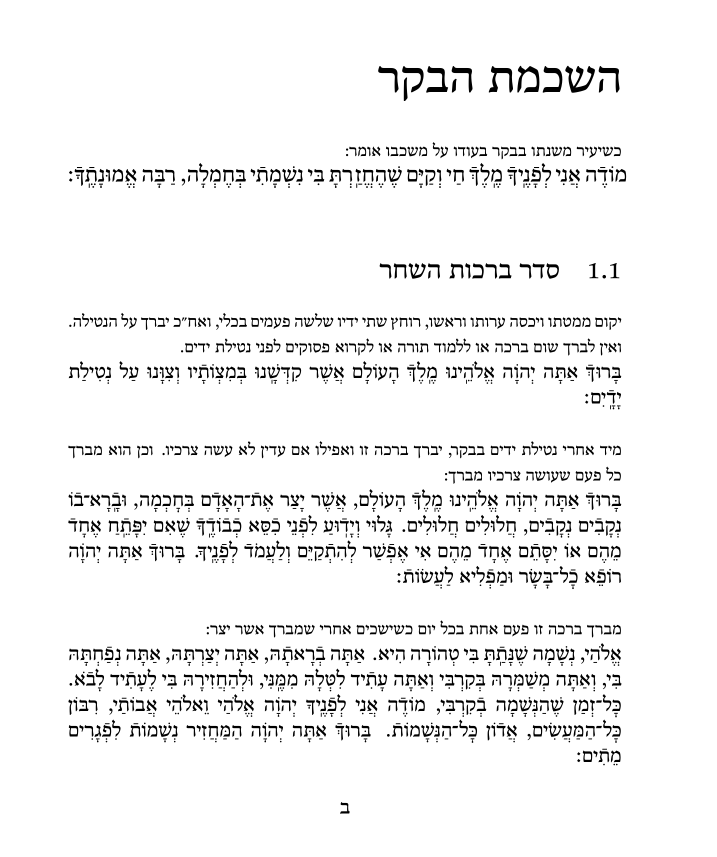
\includegraphics[width=0.5\textwidth]{hashkamas_haboker}
		\caption{First page of the Siddur showing chapter and section headings.}
	\end{figure}
	\begin{figure}[h!]
		\centering
		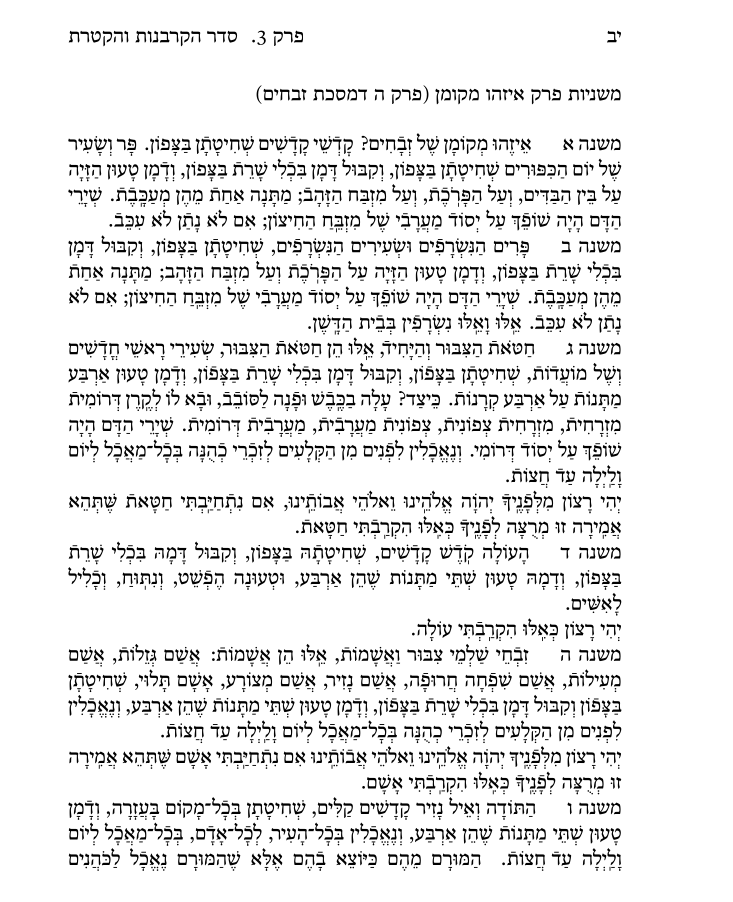
\includegraphics[width=0.5\textwidth]{eizehu_mekoman}
		\caption{Example of mishnayos in the Siddur.}
	\end{figure}
	\begin{figure}[h!]
		\centering
		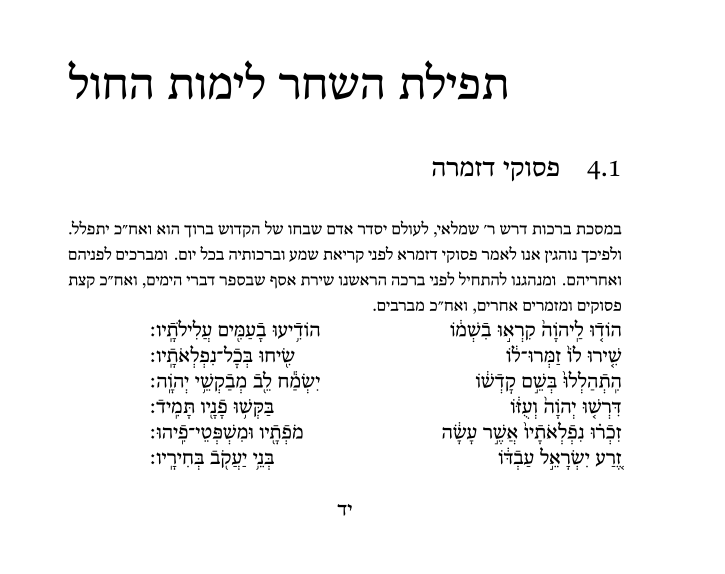
\includegraphics[width=0.5\textwidth]{pesukei_dezimra}
		\caption{Example of tzuras  hashira for Pesukeu Dezimra along with a chapter heading.}
	\end{figure}
	\begin{figure}[h!]
		\centering
		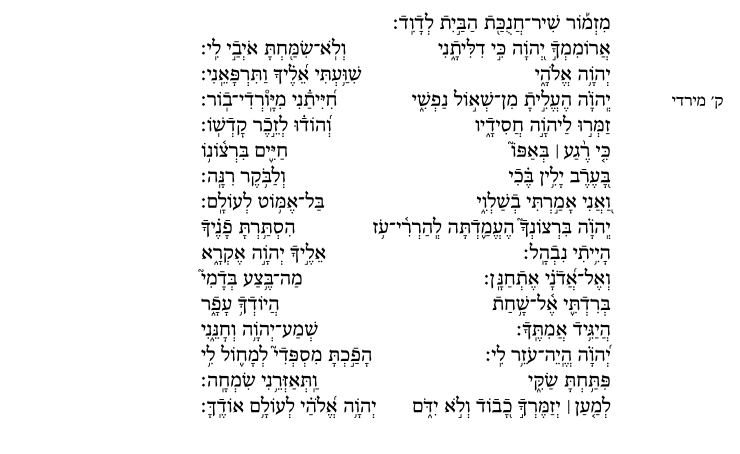
\includegraphics[width=0.5\textwidth]{tehillim_30}
		\caption{Another example of tzuras hashira for Pesukei Dezimra along with an example of how I've handled kri/ksiv in my Siddur.}
	\end{figure}
	\begin{figure}[h!]
		\centering
		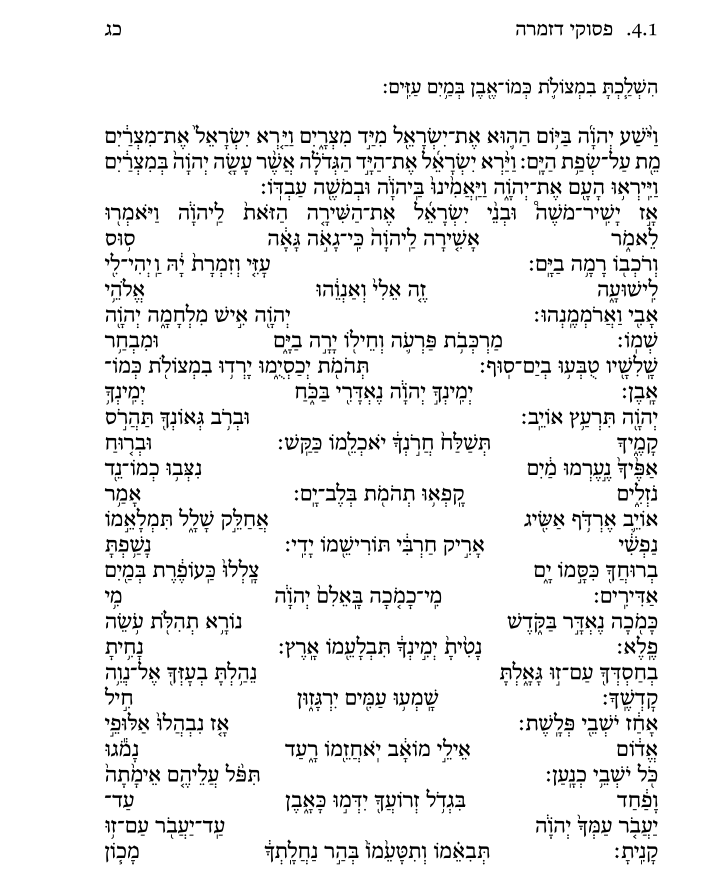
\includegraphics[width=0.5\textwidth]{shiras_hayam}
		\caption{Special tzuras hashira for Shiras HaYam.}
	\end{figure}
	\begin{figure}[h!]
		\centering
		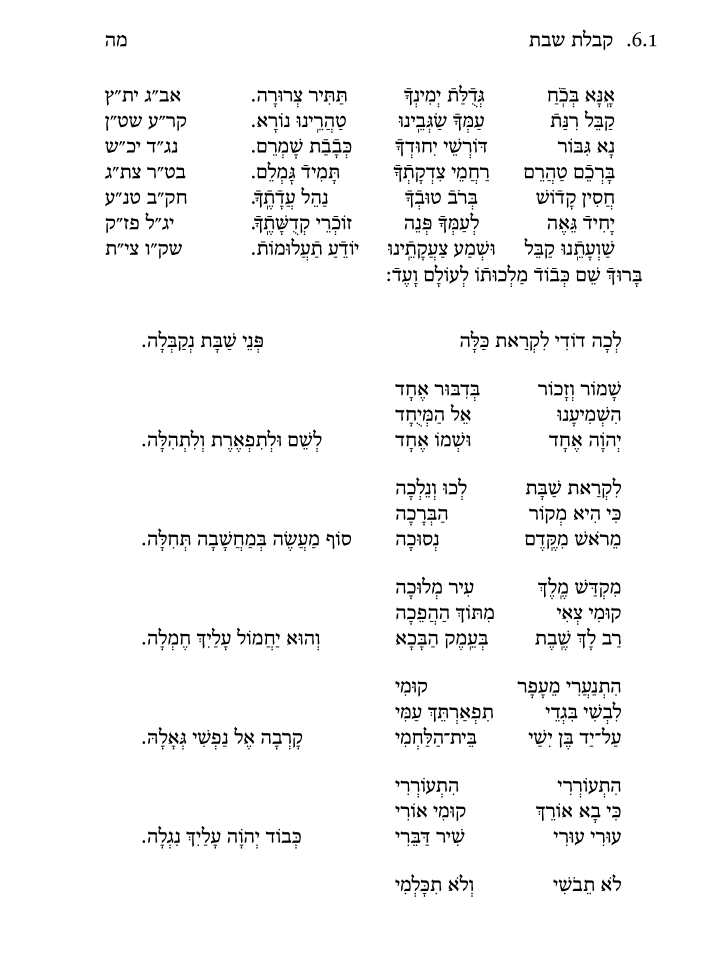
\includegraphics[width=0.5\textwidth]{lecha_dodi}
		\caption{Example of use of longpackage.sty for tysetting poetry, Lecha Dodi in this case, enabling the piyyut to seemlessly span multiple pages.}
	\end{figure}
\end{document}
